
\documentclass[12pt]{article}
\usepackage{a4wide}
\usepackage{amsmath,amssymb}
\usepackage{bm}
\usepackage[colorlinks]{hyperref}
\usepackage{graphicx}

\usepackage{algorithm}
\usepackage{algorithmic}

\usepackage{float}
\usepackage{bbold}
\usepackage{comment}
\usepackage{mathtools}

%\usepackage{caption,refstyle}




\usepackage[french]{babel}
\usepackage[T1]{fontenc}
\usepackage{lmodern}

\DeclareUnicodeCharacter{2009}{\,} 
\usepackage[standard]{ntheorem}


\begin{document}

\begin{titlepage}
\title{Algorithme Glouton faible par apprentissage}
\author{Congo Job
\\ Stage Master 1 de juin à juillet 2022 sous la direction de Joubine Aghili \\
 IRMA, Université de Strasbourg, France}
\date{ 22 août 2022}

\begin{figure}[b!]
\centering
\vfill
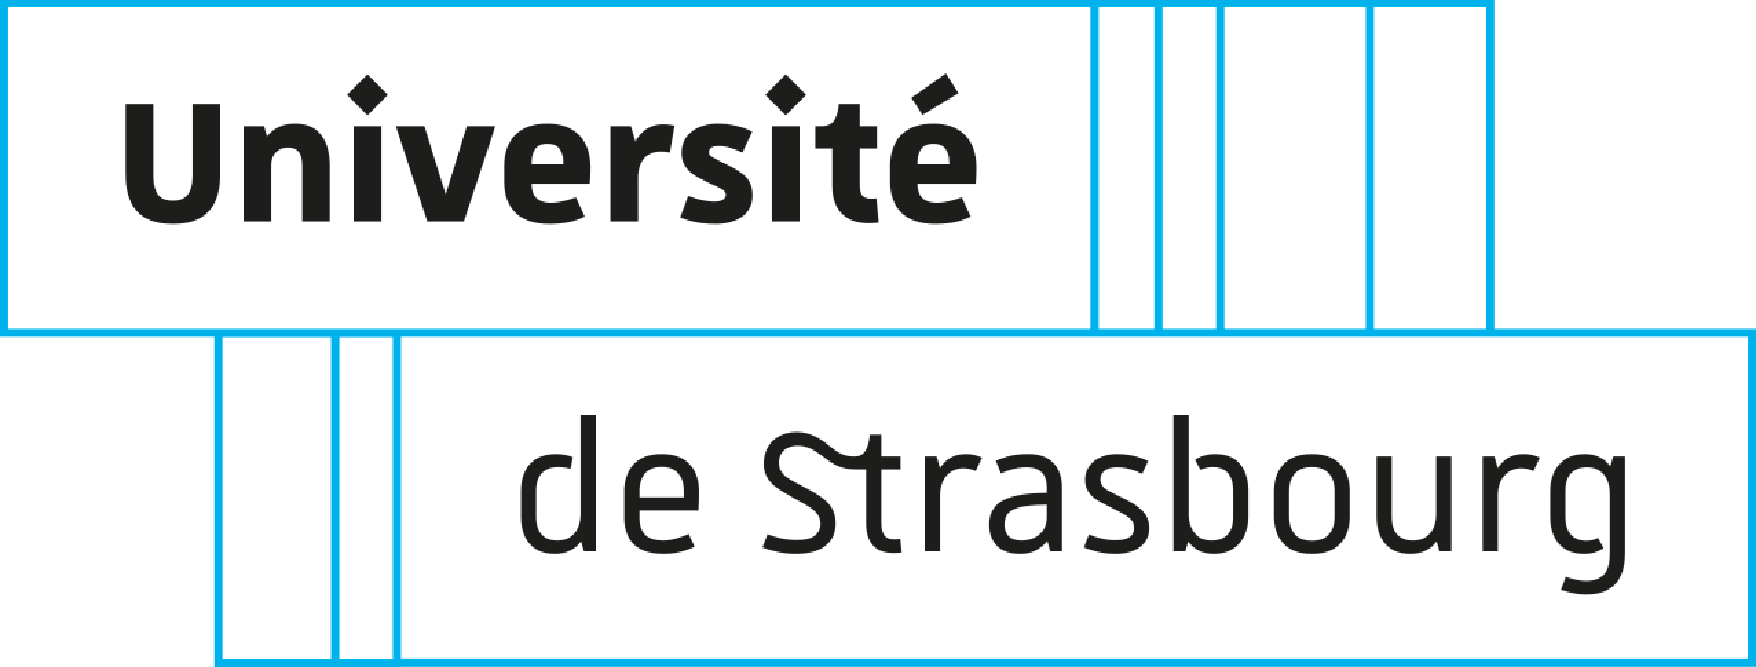
\includegraphics[scale=0.16]{logo-unistra.pdf}
\hspace{0.5 cm}
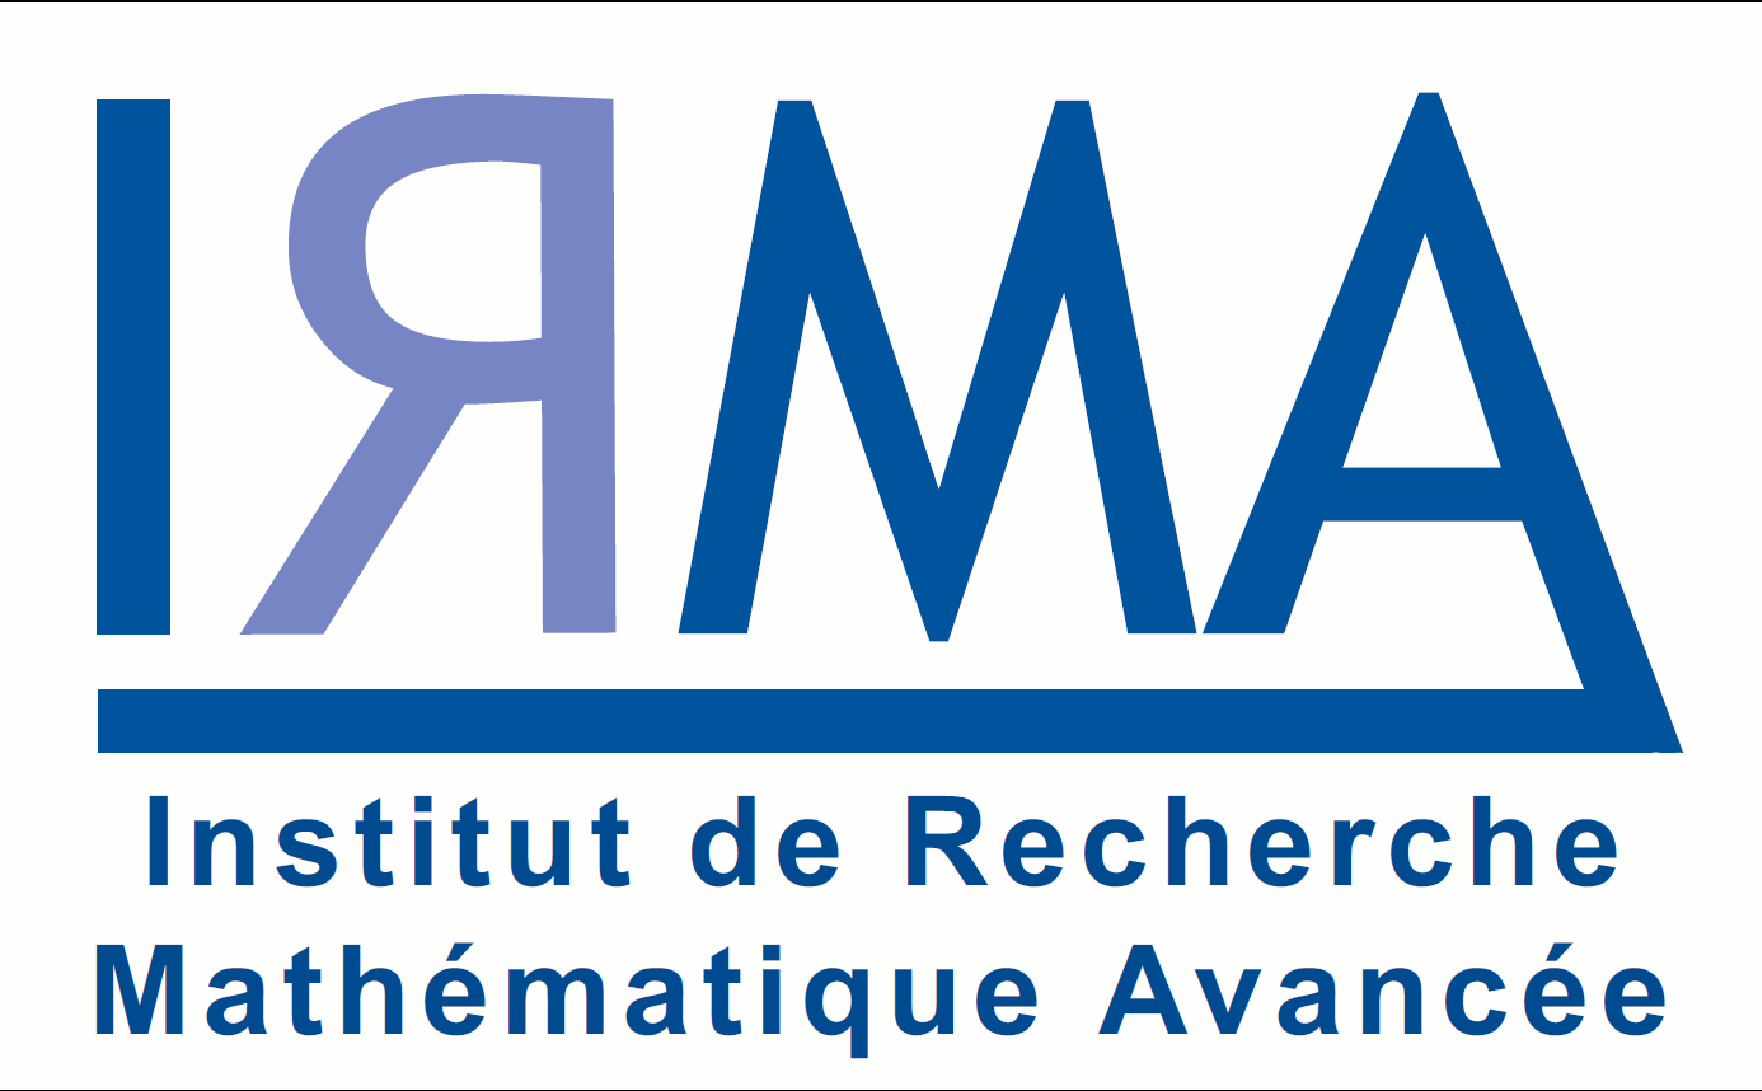
\includegraphics[scale=0.16]{logo_irma.pdf}
\hspace{0.5 cm}
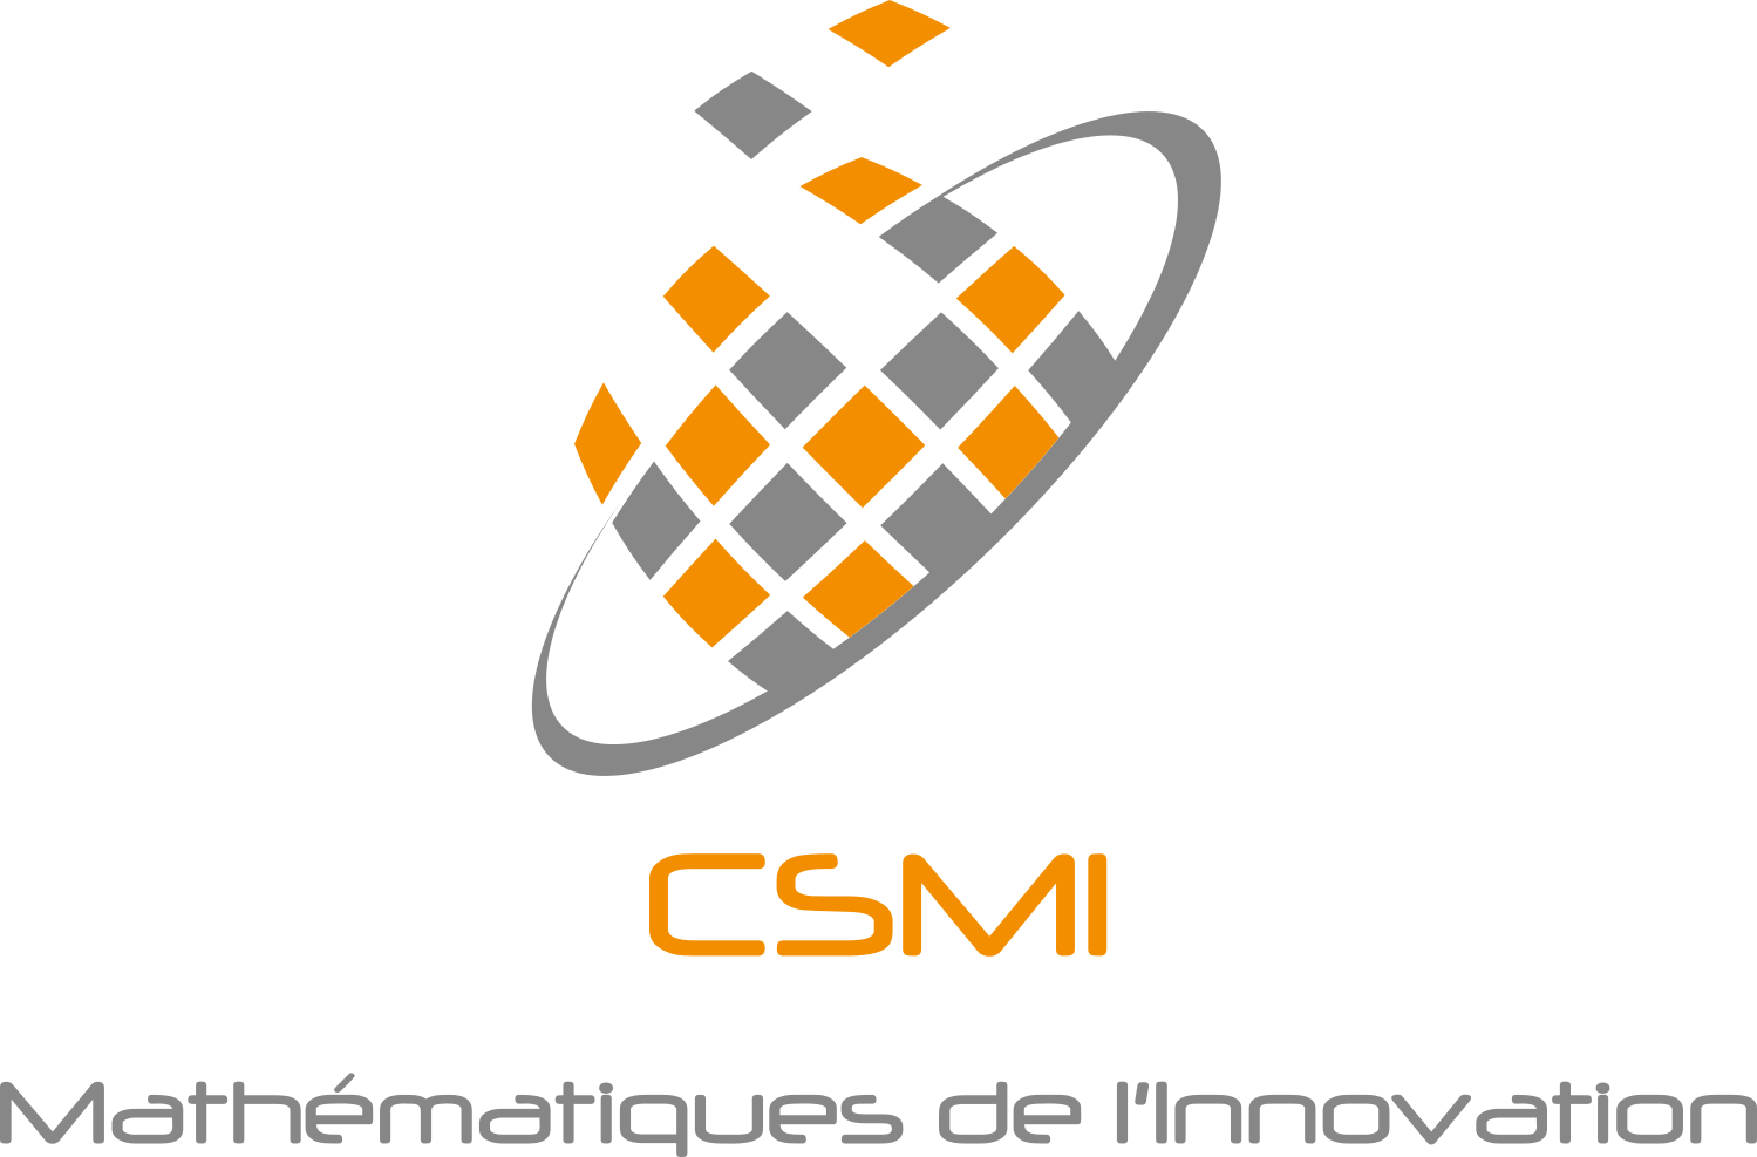
\includegraphics[scale=0.16]{logoCSMI.pdf}
\end{figure}
\end{titlepage}


\maketitle
\thispagestyle{empty}


\newpage

\tableofcontents

\newpage

\section{Introduction}



For a mathematician, Grothendieck is one of the most important mathematicians of the second half of the 20th century. He reconstructed algebraic geometry. This systematic reconstruction made it possible to solve profound problems in number theory.
However, this conference is not interested in Grothendieck's mathematics but in his life.


Alexander Grothendieck was born on March 28, 1928 in Berlin to a Russian anarchist father and a mother, a woman of letters, who had taken refuge in France.
Because of the war, he first lived with a host family in Hamburg, then he went to France.


His life can be broken down into three or four successive parts: first a mathematics researcher, then a radical ecologist and finally a hermit withdrawn from the world. I will try to present these 3 parts of his life.









\section{Mathematician}
\label{br}


1) 

When he was at school, he discovered concepts
such as length and volume, and even developed Lebesgue's integral theory.

After the baccalaureate, he became a pupil of Schwartz and Dieudonné in functional analysis. Dieudonné found him a little pretentious and asked him to work on questions that neither he nor Schwartz had been able to solve. 
They gave him 14 questions and problems, and after a few weeks he had solved half of them.
From then on, he became well known among mathematicians.

Grothendieck was awarded a doctorate for his work on topological vector spaces.



2) Largely under the influence of Serre, he turned to algebraic geometry in 1954.  At that time, the most 
 most spectacular result in the field was the Riemann-Roch-Hirzebruch theorem. He proved this theorem in the general case. He became a celebrity in the mathematical community.

3) Two years after his interest in algebraic geometry was aroused, Grothendieck found a large-scale generalisation and a whole new way of working.
large-scale generalisation and a completely new proof, which has perhaps remained his most important 
achievement in mathematics.


4)At the IHES, with Dieudonné, his former professor, he spent 15 years reconstructing algebraic geometry, in particular with the Eléments de Géométrie Algébrique (EGA) and the Séminaire de Géométrie Algébrique (SGA).

5 optional) Grothendieck had a singular approach to mathematics: rather than trying to solve difficult problems, he aimed for a deep understanding of the underlying structures, convinced that the solutions would follow naturally.
Grothendieck worked hard, doing twelve hours of mathematics a day. hours of mathematics a day.


6) However, conflicts with Motchane, the founder of the IHES institute, and with his colleague René Thom caused him to leave the mathematical community in 1970.




















\section{Ecolo}
\label{br}



Grothendieck found an occupation that he considered more important than mathematics. He became involved in environmental protection, the ecological movement, and other causes. His main involvement was with the group 'Survivre et Vivre', an international movement for the survival of the human species, fighting against ecological threats and military conflicts. 
He was able to recruit other mathematicians. But the indifference of scientists forced him to withdraw from society.





\section{Hermit}
\label{br}


In Recoltes et Semailles we find texts on mathematics and its particular poetry, reflections on ecology, meditations of a spiritual nature and a fair amount of settling of scores. 


Grothendieck's book 'La Clef des Songes' is little known and difficult to classify. It is neither a scientific work, nor an autobiography, nor a work of fiction. Grothendieck talks a lot about dreams and gives a possible interpretation of them, always in a poetic way.


\section{Conclusion}






\begin{thebibliography}{9}

\bibitem{Gianluigi Rozza}
Gianluigi Rozza.  \emph{An introduction to reduced basis method for parametrized PDEs, ResearchGate}

\end{thebibliography}

\end{document}